\documentclass[11pt,]{article}
\usepackage{lmodern}

\usepackage{amssymb,amsmath}
\usepackage{ifxetex,ifluatex}
\usepackage{fixltx2e} % provides \textsubscript
\ifnum 0\ifxetex 1\fi\ifluatex 1\fi=0 % if pdftex
  \usepackage[T1]{fontenc}
  \usepackage[utf8]{inputenc}
\else % if luatex or xelatex
  \ifxetex
    \usepackage{mathspec}
    \usepackage{xltxtra,xunicode}
  \else
    \usepackage{fontspec}
  \fi
  \defaultfontfeatures{Mapping=tex-text,Scale=MatchLowercase}
  \newcommand{\euro}{€}
\fi
% use upquote if available, for straight quotes in verbatim environments
\IfFileExists{upquote.sty}{\usepackage{upquote}}{}
% use microtype if available
\IfFileExists{microtype.sty}{%
\usepackage{microtype}
\UseMicrotypeSet[protrusion]{basicmath} % disable protrusion for tt fonts
}{}
\usepackage[lmargin=5cm,rmargin=2.5cm,tmargin=2.5cm,bmargin=2.5cm]{geometry}

%% citation setup

\usepackage{csquotes}

\usepackage[backend=biber, maxbibnames = 99, style = apa]{biblatex}
\setlength\bibitemsep{1.5\itemsep}
\bibliography{references.bib}
\usepackage{longtable,booktabs}
\usepackage{graphicx}
\makeatletter
\def\maxwidth{\ifdim\Gin@nat@width>\linewidth\linewidth\else\Gin@nat@width\fi}
\def\maxheight{\ifdim\Gin@nat@height>\textheight\textheight\else\Gin@nat@height\fi}
\makeatother
% Scale images if necessary, so that they will not overflow the page
% margins by default, and it is still possible to overwrite the defaults
% using explicit options in \includegraphics[width, height, ...]{}
\setkeys{Gin}{width=\maxwidth,height=\maxheight,keepaspectratio}
\ifxetex
  \usepackage[setpagesize=false, % page size defined by xetex
              unicode=false, % unicode breaks when used with xetex
              xetex]{hyperref}
\else
  \usepackage[unicode=true]{hyperref}
\fi
\hypersetup{breaklinks=true,
            bookmarks=true,
            pdfauthor={Jonathan Berrisch, Timo Rammert},
            pdftitle={A Forecasting Study on Global Wine Sales},
            colorlinks=true,
            citecolor=blue,
            urlcolor=blue,
            linkcolor=magenta,
            pdfborder={0 0 0}}
\urlstyle{same}  % don't use monospace font for urls
\setlength{\parindent}{0pt}
\setlength{\parskip}{6pt plus 2pt minus 1pt}
\setlength{\emergencystretch}{3em}  % prevent overfull lines
\setcounter{secnumdepth}{5}

%%% Use protect on footnotes to avoid problems with footnotes in titles
\let\rmarkdownfootnote\footnote%
\def\footnote{\protect\rmarkdownfootnote}

%%% Change title format to be more compact
\usepackage{titling}

% Create subtitle command for use in maketitle
\newcommand{\subtitle}[1]{
  \posttitle{
    \begin{center}\large#1\end{center}
    }
}

\setlength{\droptitle}{-2em}
  \title{A Forecasting Study on Global Wine Sales}
  \pretitle{\vspace{\droptitle}\centering\huge}
  \posttitle{\par}
\subtitle{Statistical Learning}
  \author{Jonathan Berrisch, Timo Rammert}
  \preauthor{\centering\large\emph}
  \postauthor{\par}
  \predate{\centering\large\emph}
  \postdate{\par}
  \date{today}


%% linespread settings

\usepackage{setspace}

\onehalfspacing

% Language Setup

\usepackage{ifthen}
\usepackage{iflang}
\usepackage[super]{nth}
\usepackage[ngerman, english]{babel}

\begin{document}

\selectlanguage{english}


%\maketitle

\begin{titlepage}
  \noindent\begin{minipage}{0.6\textwidth}
	  \IfLanguageName{english}{University of Duisburg-Essen}{Universität Duisburg-Essen}\\
	  \IfLanguageName{english}{Faculty of Business Administration and Economics}{Fakultät für Wirtschaftswissensschaften}\\
	  \IfLanguageName{english}{Chair of Econometrics}{Lehrstuhl für Ökonometrie}\\
  \end{minipage}
	\begin{minipage}{0.4\textwidth}
	  \begin{flushright}
  	  \vspace{-0.5cm}
      \IfLanguageName{english}{\includegraphics*[width=5cm]{Includes/duelogo_en.png}}{\includegraphics*[width=5cm]{Includes/duelogo_de.png}}
	  \end{flushright}
	\end{minipage}
  \\
  \vspace{1.5cm}
  \begin{center}
  \huge{A Forecasting Study on Global Wine Sales}\\
  \vspace{.25cm}
  \Large{Statistical Learning}\\
  \vspace{0.5cm}
  \large{Term Paper}\\
  \vspace{1cm}
  \large{
  \IfLanguageName{english}{Submitted to the Faculty of \\ Business Administration and Economics \\at the \\University of Duisburg-Essen}{Vorgelegt der \\Fakultät für Wirtschaftswissenschaften der \\ Universität Duisburg-Essen}\\}
  \vspace{0.75cm}
  \large{\IfLanguageName{english}{from:}{von:}}\\
  \vspace{0.5cm}
  Jonathan Berrisch, Timo Rammert\\
  \end{center}
  \vspace{4cm}

  \noindent\begin{minipage}[t]{0.3\textwidth}
  \IfLanguageName{english}{Matriculation Number}{Matrikelnummer}
  \end{minipage}
  \begin{minipage}[t]{0.7\textwidth}
  \hspace{1cm}3071485 \textbar{} 3030862
  \end{minipage}

  \noindent\begin{minipage}[t]{0.3\textwidth}
  \IfLanguageName{english}{Study Path:}{Studienfach:}
  \end{minipage}
  \begin{minipage}[t]{0.7\textwidth}
  \hspace{1cm}VWL M.Sc.
  \end{minipage}

  \noindent\begin{minipage}[t]{0.3\textwidth}
  \IfLanguageName{english}{Reviewer:}{Erstgutachter:}
  \end{minipage}
  \begin{minipage}[t]{0.7\textwidth}
  \hspace{1cm}Prof.~Dr.~Christoph Hanck
  \end{minipage}

  \noindent\begin{minipage}[t]{0.3\textwidth}
  \IfLanguageName{english}{Secondary Reviewer:}{Zweitgutachter}
  \end{minipage}
  \begin{minipage}[t]{0.7\textwidth}
  \hspace{1cm}NA
  \end{minipage}

  \noindent\begin{minipage}[t]{0.3\textwidth}
  Semester:
  \end{minipage}
  \begin{minipage}[t]{0.7\textwidth}
  \hspace{1cm}\IfLanguageName{english}{\nth{1} Semester}{1. Fachsemester}
  \end{minipage}

  \noindent\begin{minipage}[t]{0.3\textwidth}
  \IfLanguageName{english}{Graduation (est.):}{Vsl. Studienabschluss:}
  \end{minipage}
  \begin{minipage}[t]{0.7\textwidth}
  \hspace{1cm}Summer Term 2019
  \end{minipage}

  \noindent\begin{minipage}[t]{0.3\textwidth}
  \IfLanguageName{english}{Deadline:}{Abgabefrist:}
  \end{minipage}
  \begin{minipage}[t]{0.7\textwidth}
  \hspace{1cm}Aug.~27th 2019
  \end{minipage}

\end{titlepage}


\pagenumbering{Roman} 
{
\hypersetup{linkcolor=black}
\setcounter{tocdepth}{3}
\tableofcontents
}
\newpage
\listoftables
\newpage
\listoffigures
\newpage
\pagenumbering{arabic} 
\hypertarget{introduction}{%
\section{Introduction}\label{introduction}}

This paper presents a forecasting study on global wine sales. This study
is based on the friberg gronqvist wine data set which is publicly
available and was previously analyzed by {[}Textcite AER Friberg,
Grönqvist{]}. Recent technological advancements led to an significant
increase in techniques that are computationally demanding and are
potentially outperforming classical statistical methods, especially in
terms of forecasting. Those techniques are usually reffered as
statistical- or machine learning methods.

We present various models which are increasingly complex. Those models
potentially gain forecasting power while losing interpretability. The
applied models range from linear regressions to tree based methods like
Random Forests and Boosting. The goal is to develop the best possible
model to forecast wine sales in litre. Although the main goal is an
accurate forecast, some of the methods used in this paper can also be
used to check whether there is an impact of expert reviews on the sales.
This effect of expert opinion on consumer demand is a quite popular
topic. E.g. {[}Textcite Hilger, Rafert, Villas Boas{]} use a field
experiment to study a review-based demand effect using wine score labels
in a retail grocery chain.

The remainder of this paper is structured as follows. Chapter 2 gives an
overview about the dataset and the preprocessing. Chapter 3 describes
the validation approach. Chapter 4 presents the models and their
specification. Chapter 5 provides the results, a conclusion and some
ideas for future research.

\hypertarget{data-and-variables}{%
\section{Data and Variables}\label{data-and-variables}}

The datset contains 145179 observations with 59 variables. The variables
include the name of the wine, the country of origin, its price, the
amount sold per week in litre, the taste segment and variables related
to different reviews among others. We need to omit two variables
beforehand, namely \enquote{time\_segm\_price} and \enquote{artikpr},
because those are combinations of other existing variables. Hence
inclusion would lead to the problem of multicollinearity. After omitting
those two we have left the following types of variables:

\begin{longtable}[]{@{}rrrr@{}}
\toprule
Date & factor & logical & numeric\tabularnewline
\midrule
\endhead
1 & 8 & 19 & 29\tabularnewline
\bottomrule
\end{longtable}

Figure 1 depicts the amount of missing values in each variable. The
number of complete cases would be zero without further selection.
Therefore we exclude every variable with a ratio of missing values that
exceeds \(50\%\). In consequence 41416 observations with 45 variables
are used for building the forecasting models.

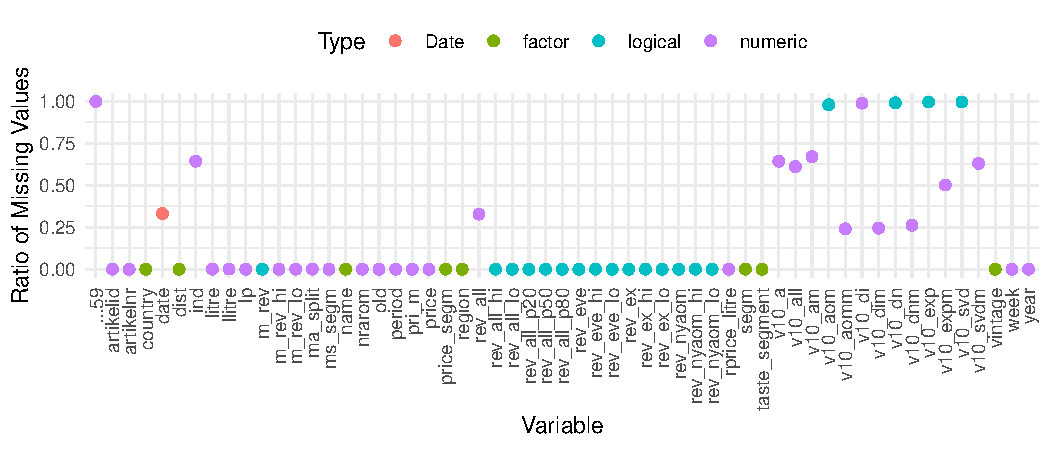
\includegraphics{../00_data/output_paper/02_missings.pdf}

Figure XY depicts the distribution of the litre variable which is the
dependend variable in our models. One can see that the observations are
heavily skewed. The Maximum is at \(184200\) litres sold weekly while
it's minimum is near zero with only \(0.75\) litres sold per week.

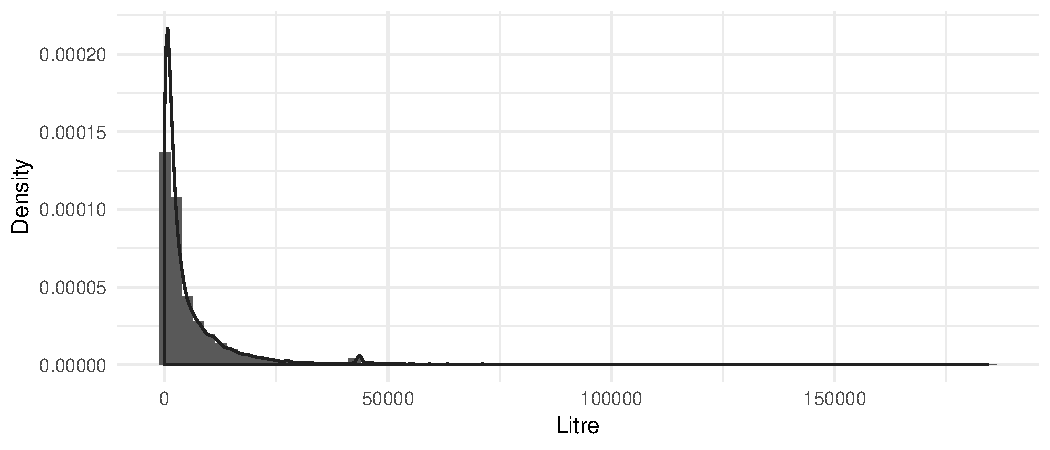
\includegraphics{../00_data/output_paper/04_hist_litre.pdf}

\hypertarget{validation-approach}{%
\section{Validation Approach}\label{validation-approach}}

Sampling may influence the model selection process because a sample
could be in favor of one specific method while another sample could lead
to different results. Therefore we validate the results of each method
using a 5-fold cross-validation. This reduces the influence of sampling
when building a training and test set while it's computationally
feasible.

In order to compute a prediction it's necessary that the test set
includes, at least all, features of the training set. Due to the high
number of levels in the countries and name variable this was not always
the case. Therefore we are using only the intersection of training and
test features to be included in the estimation.

\hypertarget{analysis}{%
\section{Analysis}\label{analysis}}

\hypertarget{mean-regression-and-linear-regression}{%
\subsection{Mean Regression and Linear
Regression}\label{mean-regression-and-linear-regression}}

At first a mean regression and a linear regression are calculated. Those
models are representing the baseline. For comparison of the different
models, the Root Mean Sqaured Error (RMSE)
\[\sqrt{\frac{1}{n}\sum_{i = 1}^{n}\left(y_i-\hat{y}_i\right)^2}\] is
calculated.

The mean regression yields an average RMSE of \(\approx 13340\) litre
sold per week. The linear regression where all variables are included
yields an average RMSE of \(\approx 5572\). The latter results is
probably influenced by overfitting. To cope with this problem we are
using variable selection and dimension reduction methods which are
discussed in the proceeding sections.

\hypertarget{lasso}{%
\subsection{Lasso}\label{lasso}}

The Least Absolute Shrinkage and Selection Operator (Lasso) is a method
combining shrinkage of the coefficent estimates to do variable
selection. It fits a linear model that is constrained by a penalty term,
i.e.~the lasso coefficients minimize:

\[
\sum_{i=1}^{n}(y_i - \beta_0 - \sum_{j=1}^{p}\beta_jx_{ij})+\lambda\sum_{j=1}^{p}|\beta_j|.
\]

Figure XY depicts the relation between lambda and the coefficients. The
crossvalidated log lambda, which minimizes the test error is
\(\approx 5812.24\). At that level a total of \(\approx 666.6\) out of
\(713\) coefficients are nonzero. The other coefficients are exactly
zero due to the sparsitiy property of the lasso estimator. Furthermore,
the plot includes abbreviated variable names of the 10 biggest
coefficients. All of those coefficients are dummys for specific wine
names. The average RMSE of the lasso approach is \(\approx 5547.76\).
This is a slight improvement above the linear baseline model. The lasso
does not significantly reduce the feature set. It shows, that the name
variable is the most important explaining the sold litre per week,
followed by the Vintage, the Region, the taste segment and the Country
of the wine. The least influence important variables are the review
variables which are not present in the 400 biggest coefficients.

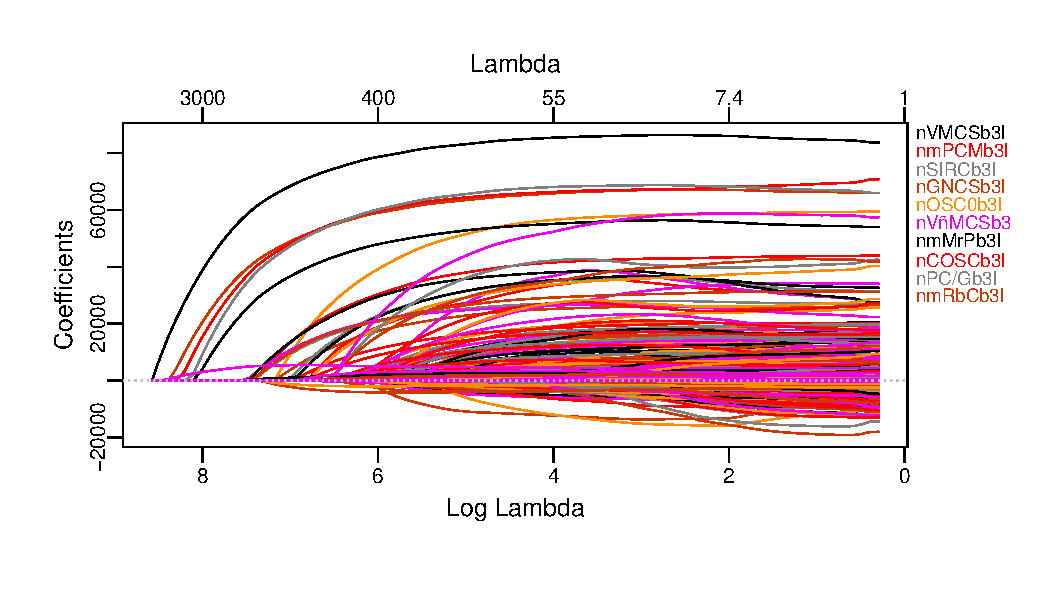
\includegraphics{../00_data/output_paper/06_lasso_vars.pdf}

\hypertarget{pls-and-pcr}{%
\subsection{PLS and PCR}\label{pls-and-pcr}}

\hypertarget{splines}{%
\subsection{Splines}\label{splines}}

\hypertarget{decision-tree-methods}{%
\subsection{Decision tree methods}\label{decision-tree-methods}}

Tree-based methods utilze decision rules to split the feature space into
a number of different regions. ``Since the set of splitting rules used
to segment the predictor space can be summarized in a tree, these type
of approaches are known as decision tree methods'' {[}Textcite Hastie,
p.~303{]}. The base of tree-based methods are regression trees For
improvement of the predictive power of these methods, while losing
interpretability, one can combine different regression trees for a
single prediction. Those approaches, including bagging, random forests
and boosting, are described in more detail when being applied.

\hypertarget{regression-tree}{%
\subsubsection{Regression Tree}\label{regression-tree}}

\hypertarget{pruned-tree}{%
\subsubsection{Pruned Tree}\label{pruned-tree}}

\hypertarget{bagging}{%
\subsubsection{Bagging}\label{bagging}}

\hypertarget{random-forest}{%
\subsubsection{Random Forest}\label{random-forest}}

\hypertarget{boosting}{%
\subsubsection{Boosting}\label{boosting}}

\hypertarget{conclusion}{%
\section{Conclusion}\label{conclusion}}

\pagebreak

\hypertarget{citations}{%
\subsection{Citations}\label{citations}}

\pagebreak

\hypertarget{annotations}{%
\subsection{Annotations}\label{annotations}}

\hypertarget{overview-over-the-rmses}{%
\subsubsection{Overview over the RMSEs}\label{overview-over-the-rmses}}

\begin{tabular}{l|r|r}
\hline
Method & RMSE & No..of.Variables\\
\hline
Mean-Regression & 0 & 0\\
\hline
Linear Regression & 0 & 0\\
\hline
Forword Stepwise Selection & 0 & 0\\
\hline
Backward Stepwise Selection & 0 & 0\\
\hline
Regression Tree & 0 & 0\\
\hline
Pruned Tree & 0 & 0\\
\hline
Random Forest & 0 & 0\\
\hline
\end{tabular}
\renewcommand*{\mkbibnamefamily}[1]{\textbf{#1}}
\renewcommand*{\mkbibnamegiven}[1]{\textbf{#1}}
\renewcommand*{\mkbibnameprefix}[1]{\textbf{#1}}
\renewcommand*{\mkbibnamesuffix}[1]{\textbf{#1}}
\printbibliography[title=References]

\newpage
\textbf{Eidesstattliche Versicherung}

\bigskip

Ich versichere an Eides statt durch meine Unterschrift, dass ich die vorstehende Arbeit selbständig und ohne fremde Hilfe angefertigt und alle Stellen, die ich wörtlich oder annähernd wörtlich aus Veröffentlichungen entnommen habe, als solche kenntlich gemacht habe, mich auch keiner anderen als der angegebenen Literatur oder sonstiger Hilfsmittel bedient habe. Die Arbeit hat in dieser oder ähnlicher Form noch keiner anderen Prüfungsbehörde vorgelegen.

\vspace{1cm}
\rule{0pt}{2\baselineskip} %
\par\noindent\makebox[2.25in]{\indent Essen, den \hrulefill} \hfill\makebox[2.25in]{\hrulefill}%
\par\noindent\makebox[2.25in][l]{} \hfill\makebox[2.25in][c]{Jonathan Berrisch, Timo Rammert}%


\end{document}
